\chapter {Projektstruktur}
Im diesem Kapitel wird die grundlegende Projektstruktur und das Anlegen des Projektes beschrieben.

\section{Projekt anlegen}
Zu Beginn der Entwicklung war es nötig, eine Basis für die Anwendung zu schaffen. Zu dieser Basis gehörten
\begin{itemize}
\item \textbf{GitHub Repository} zur Versionsverwaltung des Codes
\item \textbf{Konfigurations-Einstellungen in package.json} zur Verwaltung der von NodeJS benötigten Pakete
\item \textbf{Konfigurations-Einstellungen in bower.json} zur Verwaltung der Pakete des FrontEnds
\item \textbf{Grundfile.js} mit allen Tasks, die während der Entwicklung und zum Deployment zum Einsatz kommen
\item \textbf{Ordner-Struktur} für Module und die eigentliche Anwendung
\end{itemize}

Dies per Hand zu machen, ist generell sehr fehleranfällig und benötigt einige Zeit. Aus diesen Gründen wurde hierbei die NodeJS-Kickstarter-Anwendung \textit{yeoman.io} verwendet.
Diese Anwendung stellt verschiedene Generatoren zur Verfügung, mit welchen sich unterschiedlichste Anwendungen kickstarten lassen. Aktuell umfasst die Generatoren-Bilbliothek mehr als 4800 verschiedene
Generator-Module.\\
Die vorliegende Anwendung wurde mithilfe des Generators \grqq angular\glqq{}  gekickstartet. \grqq angular\glqq{} ist ein offizielles vom Yeoman-Team entwickeltes Modul.
Über den Konsolenbefehl\\
\texttt{yo generator:angular App}\\
generiert Yeoman alle oben genannten Strukturen, Dateien der Boilerplate-Angular-Anwendung und Test-Methoden.
Da es sich bei AngularJS-Anwendungen meistens um Single-Page-Anwendungen handelt, ist die Ausgangdatei die \textit{index.html}-Datei im App-Ordner.
In dieser Datei werden alle JavaScript-Module und CSS-Bibliothenek zusammengeführt. Dabei zeichnet sich ein großer Vorteil von der Verwendung von Yeoman heraus:
In der HTML-Datei befinden sich Marker, mit welchen die Bereiche markiert sind, in denen JavaScripte und Stylesheets eingebaut werden. Installiert ein Benutzer über Bower neue Module, so erfolgt das Einbinden automatisch.
Gesteuert wird dieser Prozess von dem \texttt{serve}-Task in \textit{Gruntfile.js}.\\
Eine weitere sehr nützliche Funktion, ist die Möglichkeit, neue AngularJS-Module, wie z.B. Controller, Services oder Direktiven direkt über die Kommandozeile hinzuzufügen.
Die Erstellung des Kontrollers erfolgt über den Befehl \\
\texttt{yo angular:controller ControllerName}\\
Über diesen Befehl generiert Yeoman nun einen Angular-Controller, der in dem entsprechenden controller-Ordner abgelegt wird. Dieser Controller ist bereits mit der existierenden Anwendung
 verknüpft. Zudem wird das JS-File direkt in die \textit{index.html}-Datei eingebunden.\\
 Zusammengefasst erleichtert es die Verwendung eines Generators, wie in diesem Falle Yeoman, Grundlagen für eine Anwendung zu schaffen und diese in ihrer Entwicklung vornazutreiben.

\begin{figure}[H]
    \centering
    \begin{minipage}[t]{0.49\linewidth}
        \centering
        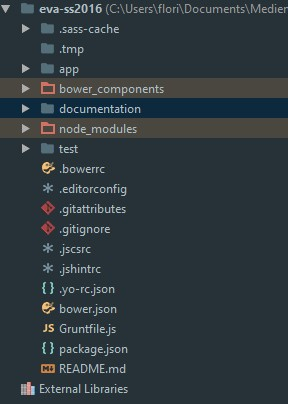
\includegraphics[width=\linewidth]{images/project_structure.jpg}
        \caption{Angelegte Projektstruktur}
        \label{project_structure}
    \end{minipage}
\end{figure}


\section{Grunt Tasks}
Wie bereits im vorausgegangenen Abschnitt erwähnt, generiert Yeoman eine JavaScript-Datei namens \textit{Gruntfile.js}. Diese beinhaltet vorgefertigte Grunt-Tasks zum Entwickeln, Test und
Deployen/Builden der Anwendung. Nachfolgend wird auf die beiden wichtigsten tasks eingegangen.

\subsection{serve}
Der \textit{serve}-Task ist der Task, der während der Entwicklung zum Einsatz kommt. Über ihn wird auf \textit{http://localhost} ein lokaler Server gestartet, auf welchem
die zu entwickelnde Anwendung erreichbar ist. Im Hintergrund wird zudem zwischen Grunt und dem Browser eine Socket-Verbindung zum Livereload aufgebaut. Der Zweck dieser Verbindung ist,
dass sobald der Entwickler in der Entwicklungsumgebung eine Änderung an Projekt-Dateien wie z.B. an JavaScript- oder Sass-Dateien Macht, automatisch ein Refresh des Browserfensters angestoßen wird.
Darüber erspart sich der Entwickler den zusätzlichen Tastendruck beim Ansehen/Testen der Seite.\\
Damit das Erkennen von Änderungen möglich ist, startet der \textit{serve}-Task Datei-Watcher, welche auf beliebige Dateien angesetzt werden können. Diese reagieren auf Änderungen und führen mit dem Datei-Typ verknüpfte Subtasks (z.B. Kompilieren von Sass-Dateien zu CSS-Dateien) aus.

\subsection{build}
Bei diesem Task handelt es sich um den Build-Task der Anwendung. Seine Aufgabe ist es, aus dem entwickelten Code eine fertige Anwendung zu generieren.
Dazu gehört das Kompilieren von Sass zu CSS, Zusammenführen von CSS- und JavaScript-Dateien, Minimieren von JavaScript (dazu kann noch ein \glqq Uglyfier \grqq{} hinzugeschaltet werden, der neben der Minimierung des Javascript-Codes diesen auch unleserlich macht), Zusammenfassen der HTML-Templates, Kopieren aller benötigten Ressourcen wie Grafiken und Fonts und letztendlich Generieren eines \textit{dist}-Ordners, der die gesamte Anwendung enthält.\\
Um die Anwendung nun zu publizieren, ist nur noch der Inhalt des \textit{dist}-Ordners nötig.